% mnras_template.tex
%
% LaTeX template for creating an MNRAS paper
%
% v3.0 released 14 May 2015
% (version numbers match those of mnras.cls)
%
% Copyright (C) Royal Astronomical Society 2015
% Authors:
% Keith T. Smith (Royal Astronomical Society)

% Change log
%
% v3.0 May 2015
%    Renamed to match the new package name
%    Version number matches mnras.cls
%    A few minor tweaks to wording
% v1.0 September 2013
%    Beta testing only - never publicly released
%    First version: a simple (ish) template for creating an MNRAS paper

%%%%%%%%%%%%%%%%%%%%%%%%%%%%%%%%%%%%%%%%%%%%%%%%%%
% Basic setup. Most papers should leave these options alone.
\documentclass[a4paper,fleqn,usenatbib]{mnras}

% MNRAS is set in Times font. If you don't have this installed (most LaTeX
% installations will be fine) or prefer the old Computer Modern fonts, comment
% out the following line
\usepackage{newtxtext,newtxmath}
% Depending on your LaTeX fonts installation, you might get better results with one of these:
%\usepackage{mathptmx}
%\usepackage{txfonts}

% Use vector fonts, so it zooms properly in on-screen viewing software
% Don't change these lines unless you know what you are doing
\usepackage[T1]{fontenc}
\usepackage{ae,aecompl}

%%%%% AUTHORS - PLACE YOUR OWN PACKAGES HERE %%%%%

% Only include extra packages if you really need them. Common packages are:
\usepackage[dvipdfmx]{graphicx}	% Including figure files
\usepackage{amsmath}	% Advanced maths commands
\usepackage{amssymb}	% Extra maths symbols
\usepackage{multicol}
\usepackage{siunitx}
\usepackage{bmpsize}
\usepackage[anythingbreaks]{breakurl}
\usepackage{subfig}
\usepackage{fancyvrb}
\usepackage{hyperref}


\def\startdata{\if@table@not@headed\kill\caption{\\%
    \@tablecaption}\endhead\hline\endfoot%
  \fi%
}

\def\enddata{% 
 \crcr 
 \noalign{\vskip .7ex}% 
 \before@enddata 
 \endtabular 
 \setbox\pt@box\lastbox 
 \pt@width\wd\pt@box\box\pt@box 
}% 


\newcommand{\aprx}{\raise.17ex\hbox{$\scriptstyle\sim$}}

%%%%%%%%%%%%%%%%%%%%%%%%%%%%%%%%%%%%%%%%%%%%%%%%%%

%%%%% AUTHORS - PLACE YOUR OWN COMMANDS HERE %%%%%

% Please keep new commands to a minimum, and use \newcommand not \def to avoid
% overwriting existing commands. Example:
%\newcommand{\pcm}{\,cm$^{-2}$}	% per cm-squared

%%%%%%%%%%%%%%%%%%%%%%%%%%%%%%%%%%%%%%%%%%%%%%%%%%

%%%%%%%%%%%%%%%%%%% TITLE PAGE %%%%%%%%%%%%%%%%%%%

% Title of the paper, and the short title which is used in the headers.
% Keep the title short and informative.
\title[spiderman]{\textsc{spiderman}: an open source code to model phase curves and secondary eclipses.}

% The list of authors, and the short list which is used in the headers.
% If you need two or more lines of authors, add an extra line using \newauthor
\author[T. Louden, L. Kreidberg]{Tom Louden$^{1}$\thanks{E-mail: t.m.louden@warwick.ac.uk} and Laura Kreidberg$^{2}$\\
$^{1}$Department of Physics, University of Warwick, Coventry, CV4 7AL, UK\\
$^{2}$Department of Astronomy, Harvard, America, America, America}

% These dates will be filled out by the publisher
\date{Accepted XXX. Received YYY; in original form ZZZ}

% Enter the current year, for the copyright statements etc.
\pubyear{2016}

% Don't change these lines
\begin{document}
\label{firstpage}
\pagerange{\pageref{firstpage}--\pageref{lastpage}}
\maketitle

% Abstract of the paper
\begin{abstract}

Presenting \textsc{spiderman}, a fast code for calculating exoplanet phase curves and secondary eclipses with arbitrary surface brightness distributions.

The development version of the code is available at \url{https://github.com/tomlouden/spiderman}.

\end{abstract}

\textsc{spiderman}

% Select between one and six entries from the list of approved keywords.
% Don't make up new ones.
\begin{keywords}
planets and satellites: individual (WASP 52b)---stars: individual (WASP 52)---techniques: spectroscopic---planets and satellites: atmospheres---celestial mechanics---atmospheric effects
\end{keywords}

%%%%%%%%%%%%%%%%%%%%%%%%%%%%%%%%%%%%%%%%%%%%%%%%%%

%%%%%%%%%%%%%%%%% BODY OF PAPER %%%%%%%%%%%%%%%%%%

\section{Introduction}\label{sec:introduction}

Secondary eclipses and phase curves can give direct insight into the thermal transport processes, and vertical structure of an exoplanet atmosphere.

Hot Jupiters are expected to be tidally locked to their parent stars, resulting in a permanent day and night side with enormous differences in incident flux. The details of the heat transport in the atmosphere will effect how efficiently energy can be transported between the two hemispheres of the planet.

General Circulation Models, GCM's, are currently the state of the art for predicting the wind patters and temperature distributions of the surface of exoplanets \citep[e.g.]{Showman2008}

An important early prediction of these GCM's was that hot, tidally locked Jupiter's would display significantly offset hotpots.

An offset hotspot can be detected though the thermal phase-curve of the planet, as the point of maximum flux will be offset from the time of secondary transit by a measurable amount. This effect can also be mimicked by a high eccentricity (CITE?). 


\citet{Zhang2016} showed that this behaviour could be captured with a simple analytical formalism.

BATMAN \citep{Kreidberg2015a}

There does not currently exist an open source code for calculating secondary eclipses and phase curves in a self consistent way, \textsc{spiderman} is designed to fulfil this role, and it is is hoped that it will be of use to the community.

\section{Method}\label{sec:method}

\begin{figure}
\begin{center}
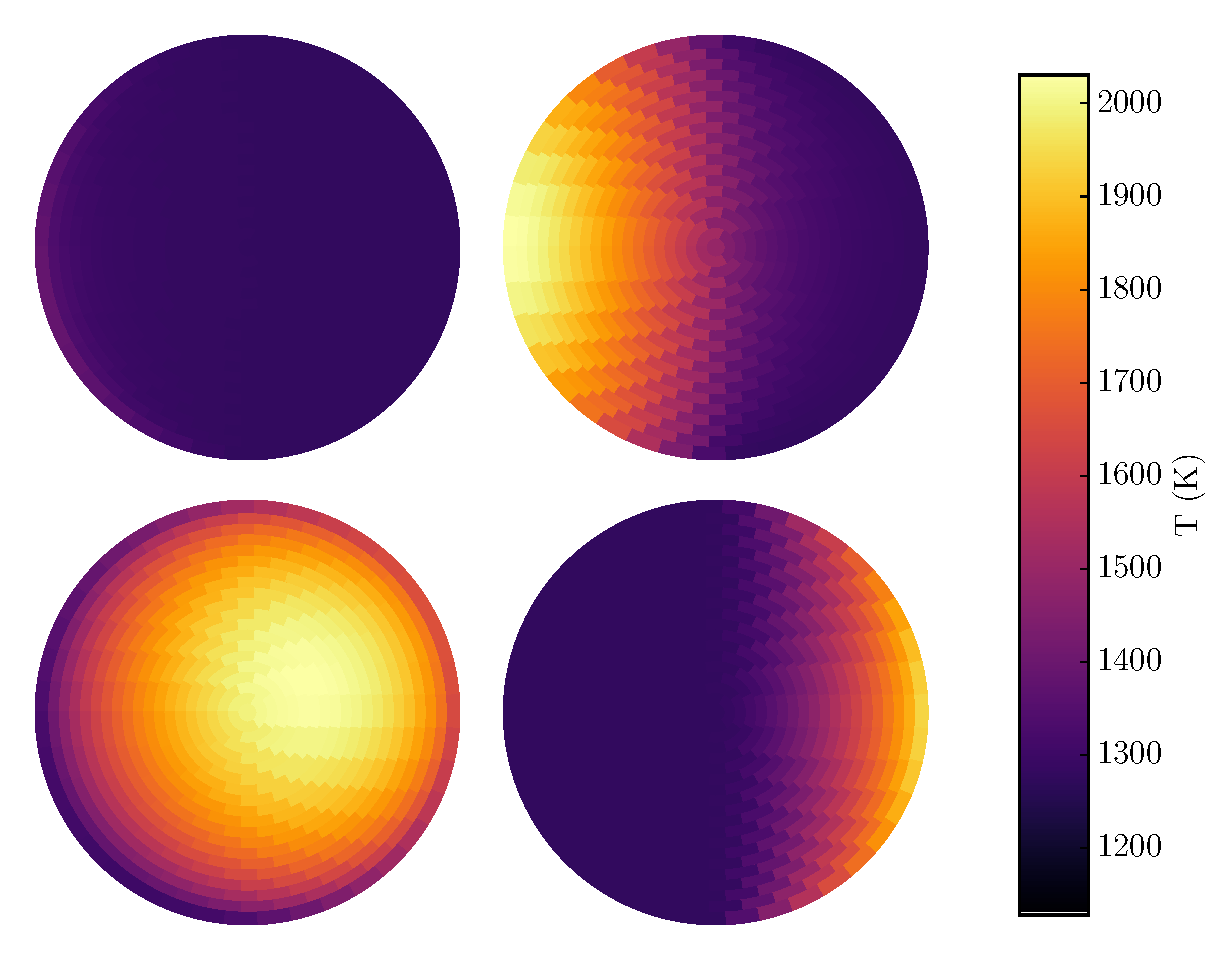
\includegraphics[width=\columnwidth]{img/zhang_quad.pdf}
\caption{This is a caption}
\label{fig:zhang_quad}
\end{center}
\end{figure}

\begin{figure}
\begin{center}
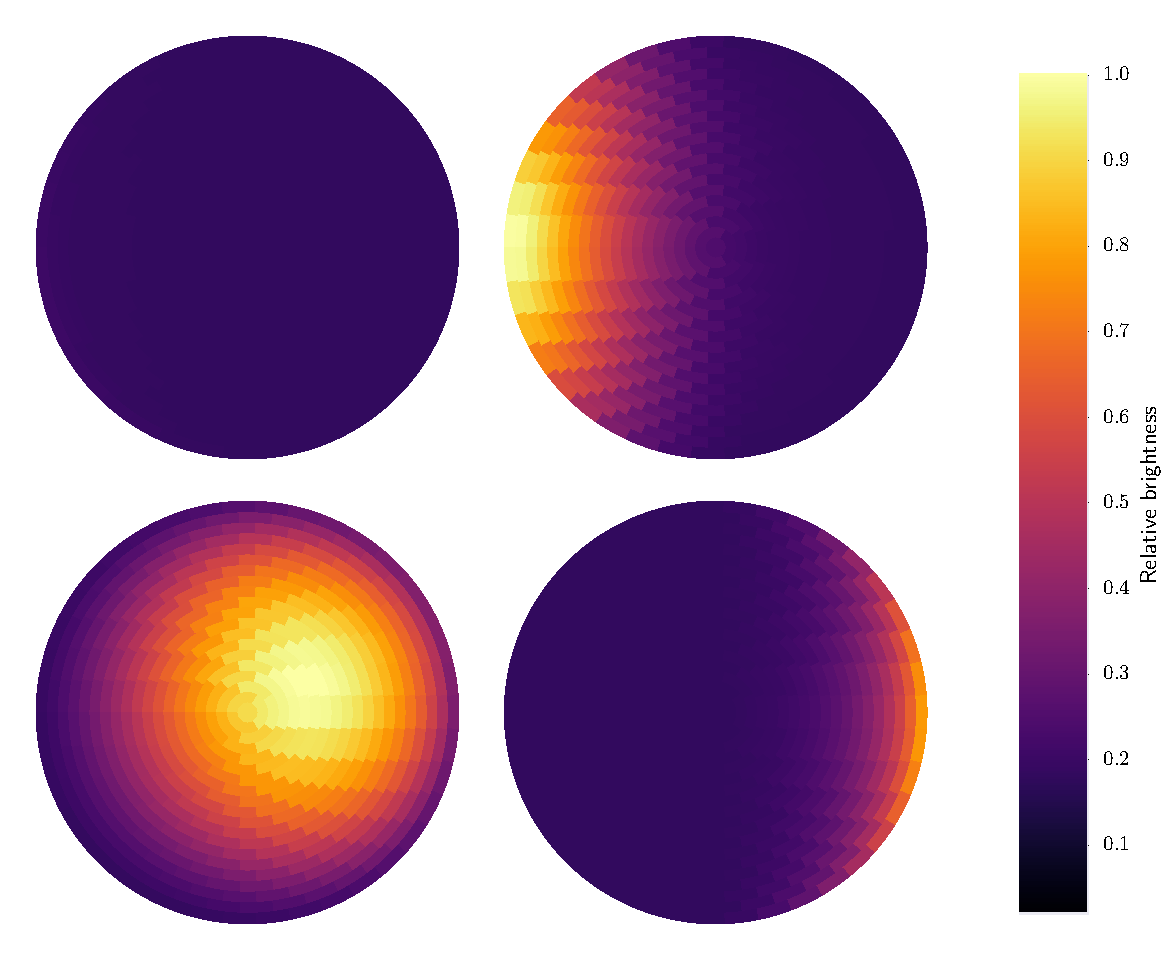
\includegraphics[width=\columnwidth]{img/zhang_quad_bright.pdf}
\caption{Same as \ref{fig:zhang_quad}, but the scale is now flux instead of temperature. A blackbody spectrum and a channel of 1.1-1.7 microns was assumed to make the conversion. The option exists to add limb darkening to this profile.}
\label{fig:zhang_quad2}
\end{center}
\end{figure}

\begin{figure}
\begin{center}
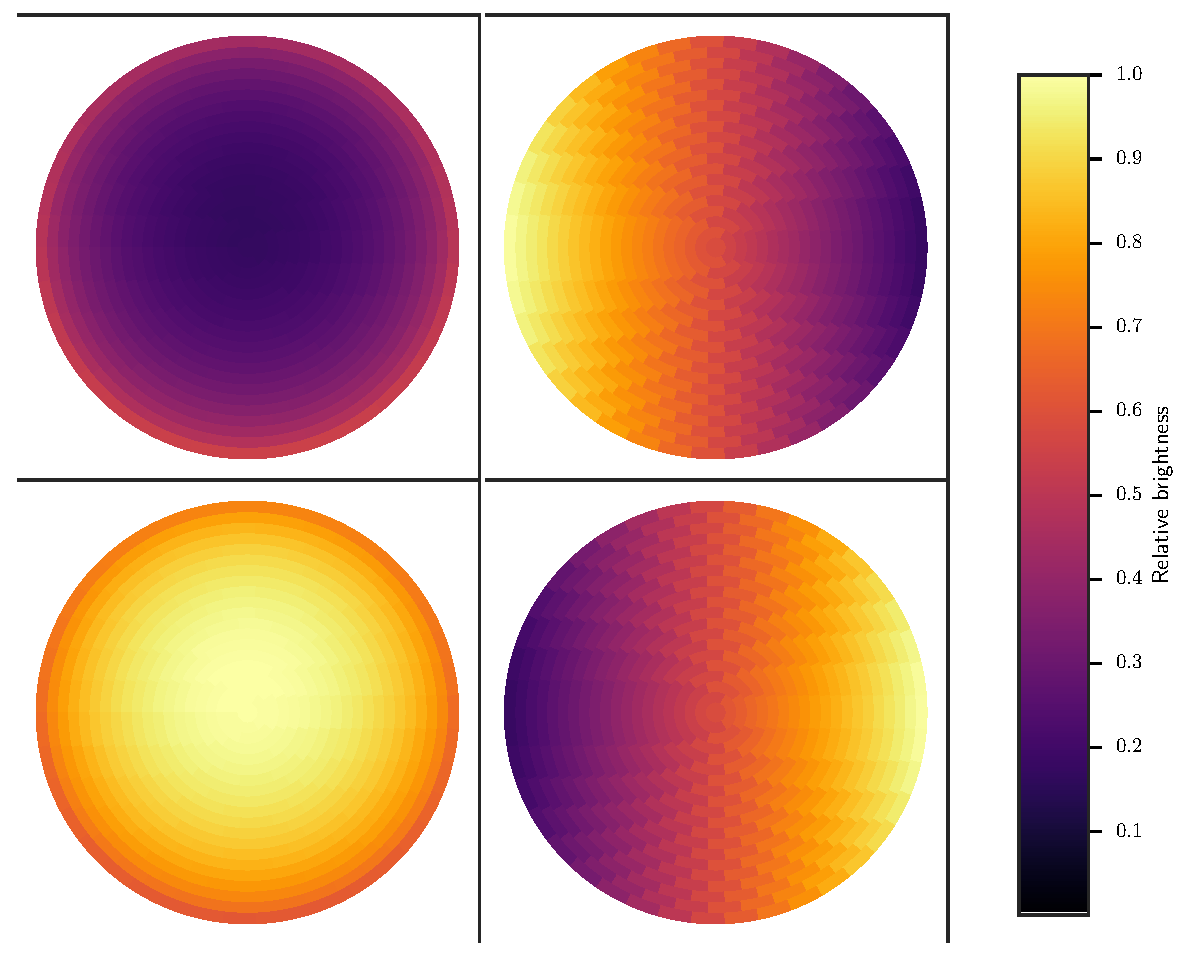
\includegraphics[width=\columnwidth]{img/sphere_quad.pdf}
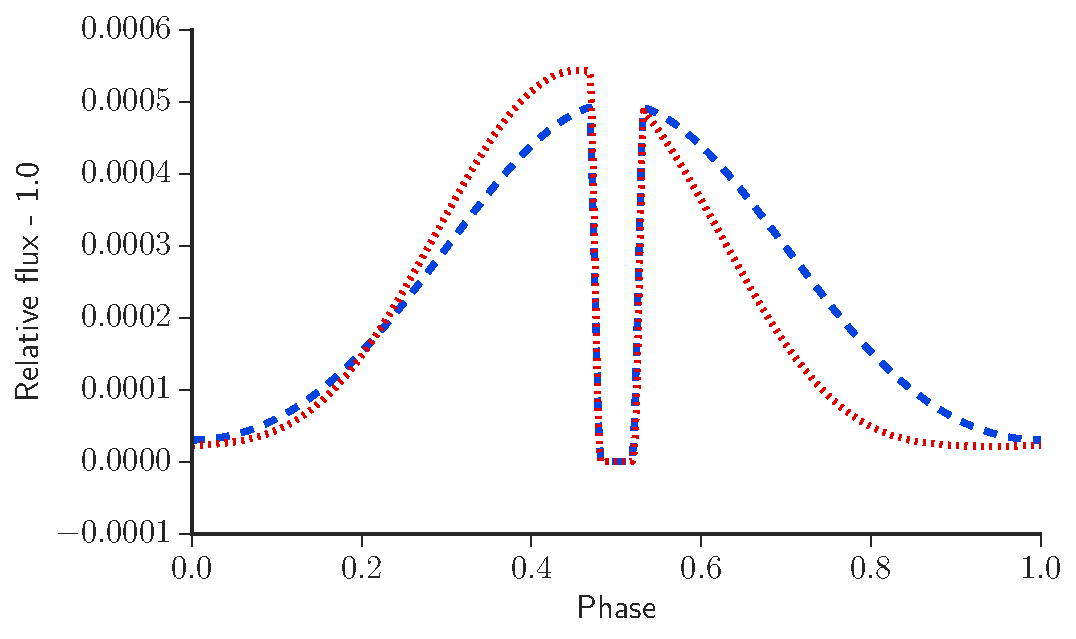
\includegraphics[width=\columnwidth]{img/spherical_lc.pdf}
\caption{A model generated using spherical harmonics}
\label{fig:harmonics}
\end{center}
\end{figure}

\begin{figure}
\begin{center}
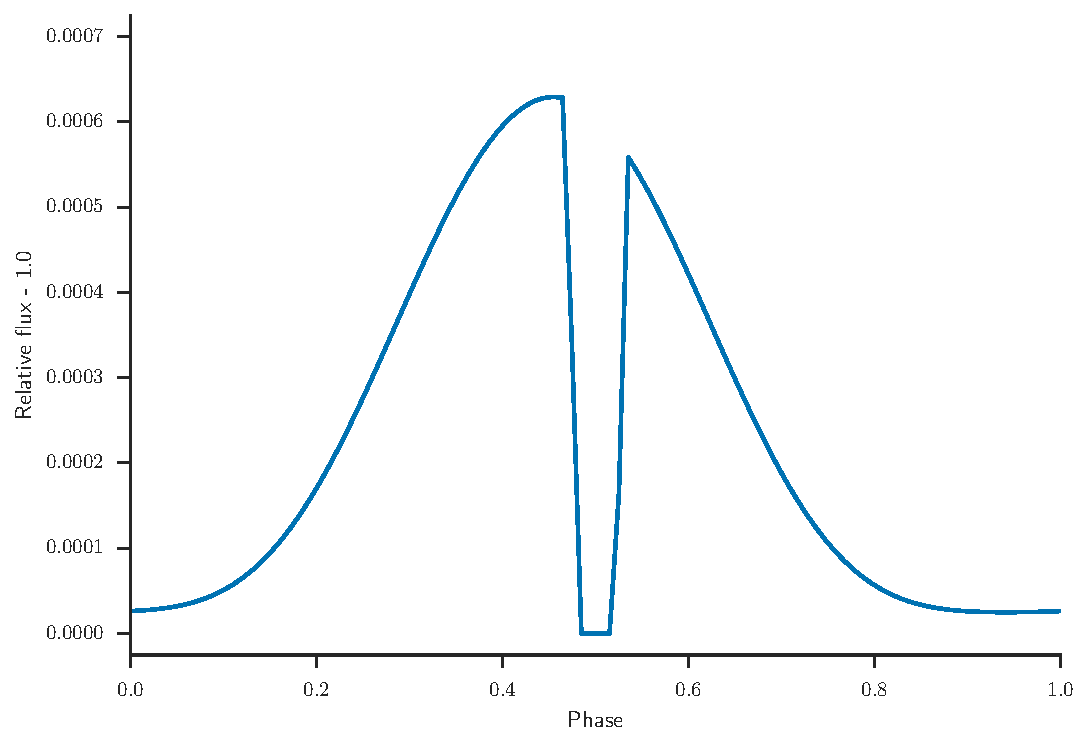
\includegraphics[width=\columnwidth]{img/zhang_lc.pdf}
\caption{This is a caption}
\label{fig:extract_region}
\end{center}
\end{figure}

\begin{figure}
\begin{center}
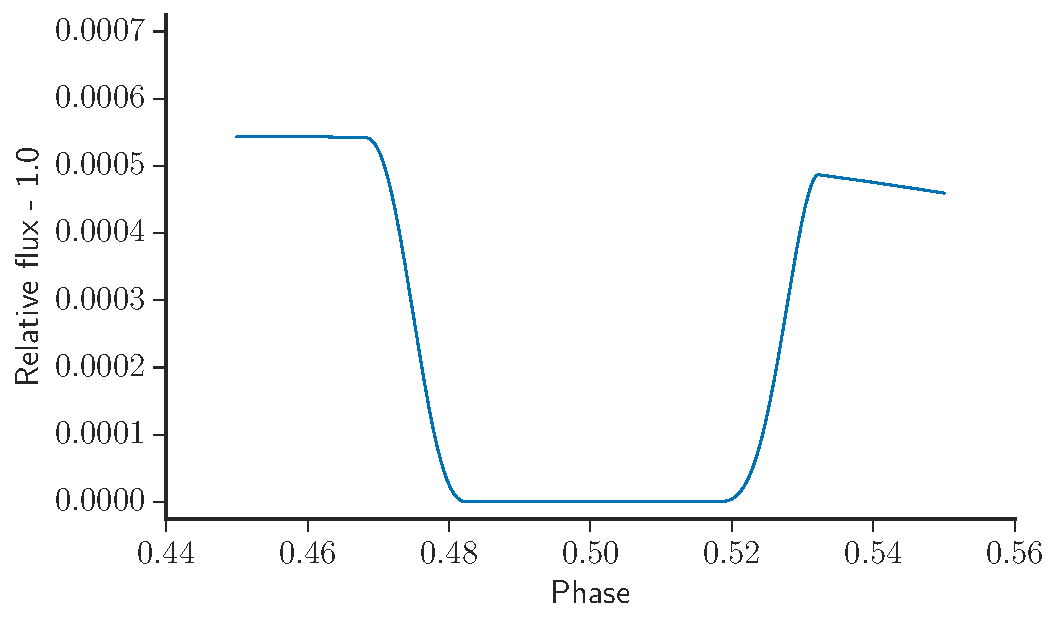
\includegraphics[width=\columnwidth]{img/zhang_lc_zoom.pdf}
\caption{This is a caption}
\label{fig:extract_region}
\end{center}
\end{figure}

\begin{figure}
\begin{center}
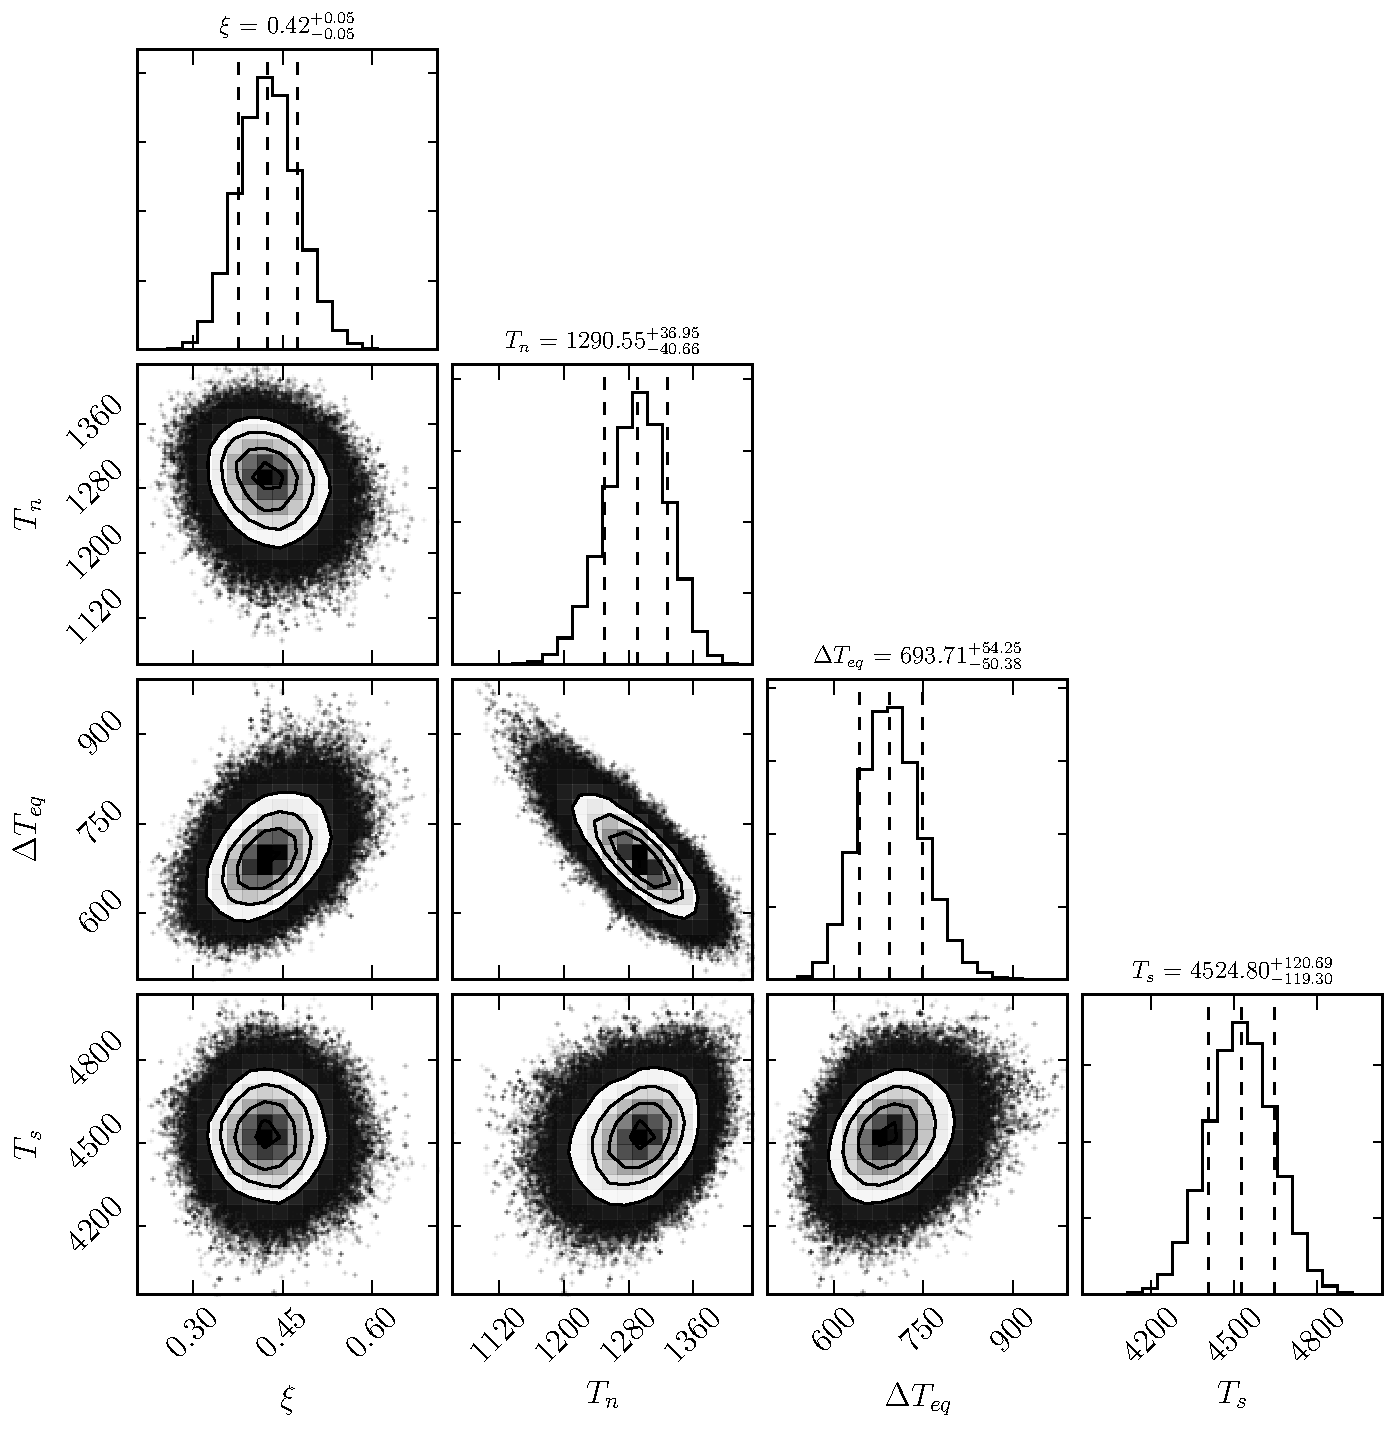
\includegraphics[width=\columnwidth]{img/free_parameterstriangle.pdf}
\caption{This is a caption}
\label{fig:extract_region}
\end{center}
\end{figure}

\begin{figure*}
\begin{center}
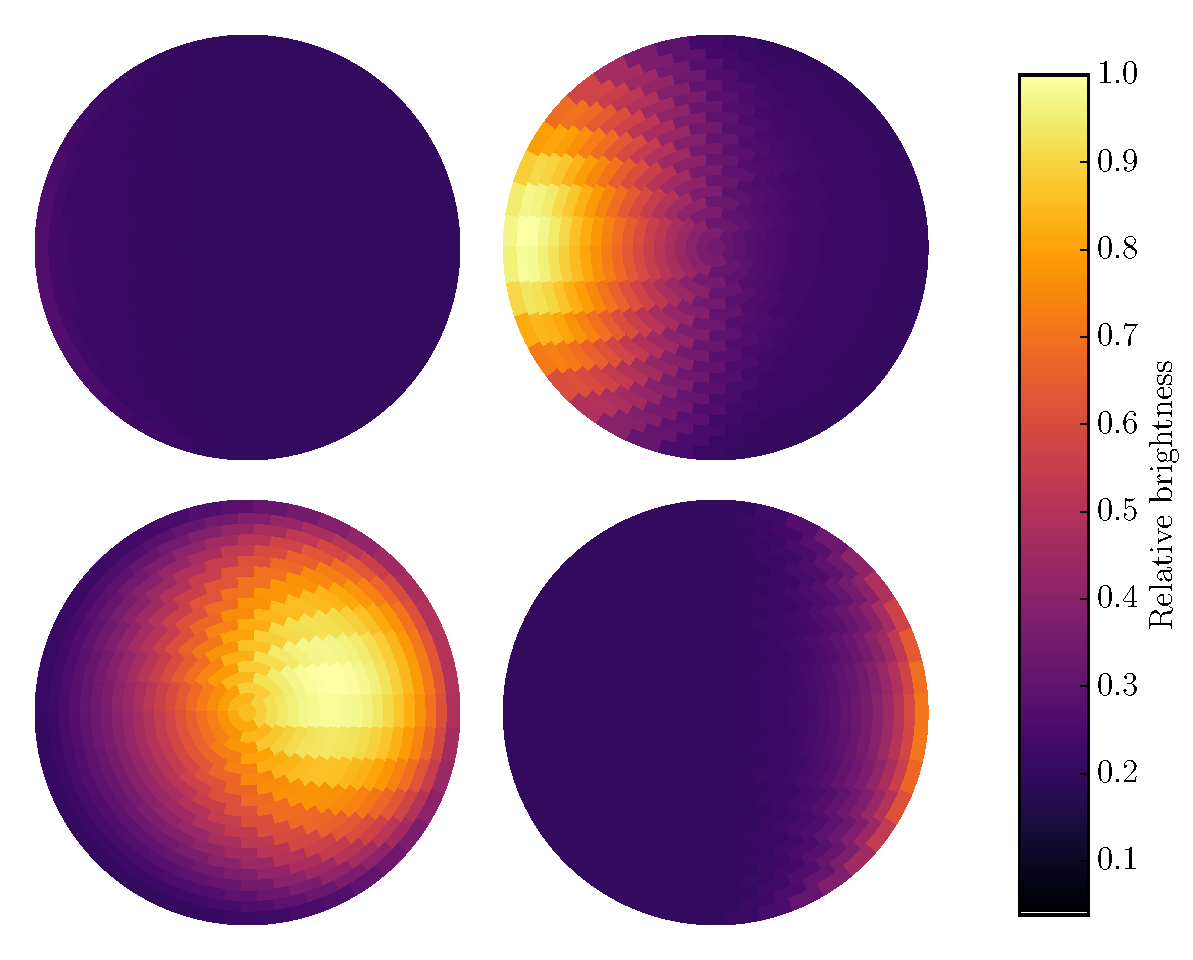
\includegraphics[width=\columnwidth]{img/free_parametersflux_map.pdf}
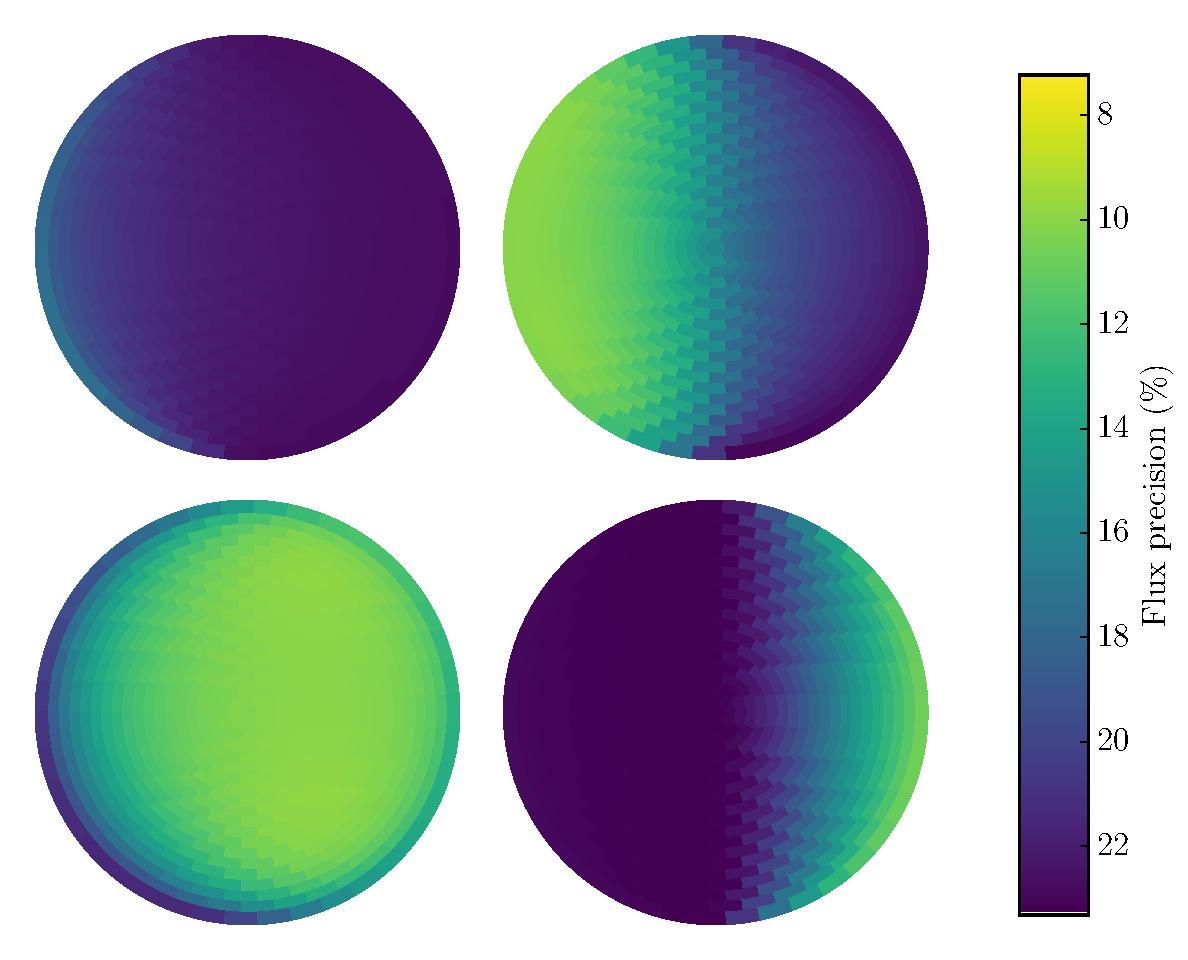
\includegraphics[width=\columnwidth]{img/free_parametersflux_errs.pdf}
\caption{left: right: the constraints on the brightness distribution.}
\label{fig:extract_region}
\end{center}
\end{figure*}

\begin{figure*}
\begin{center}
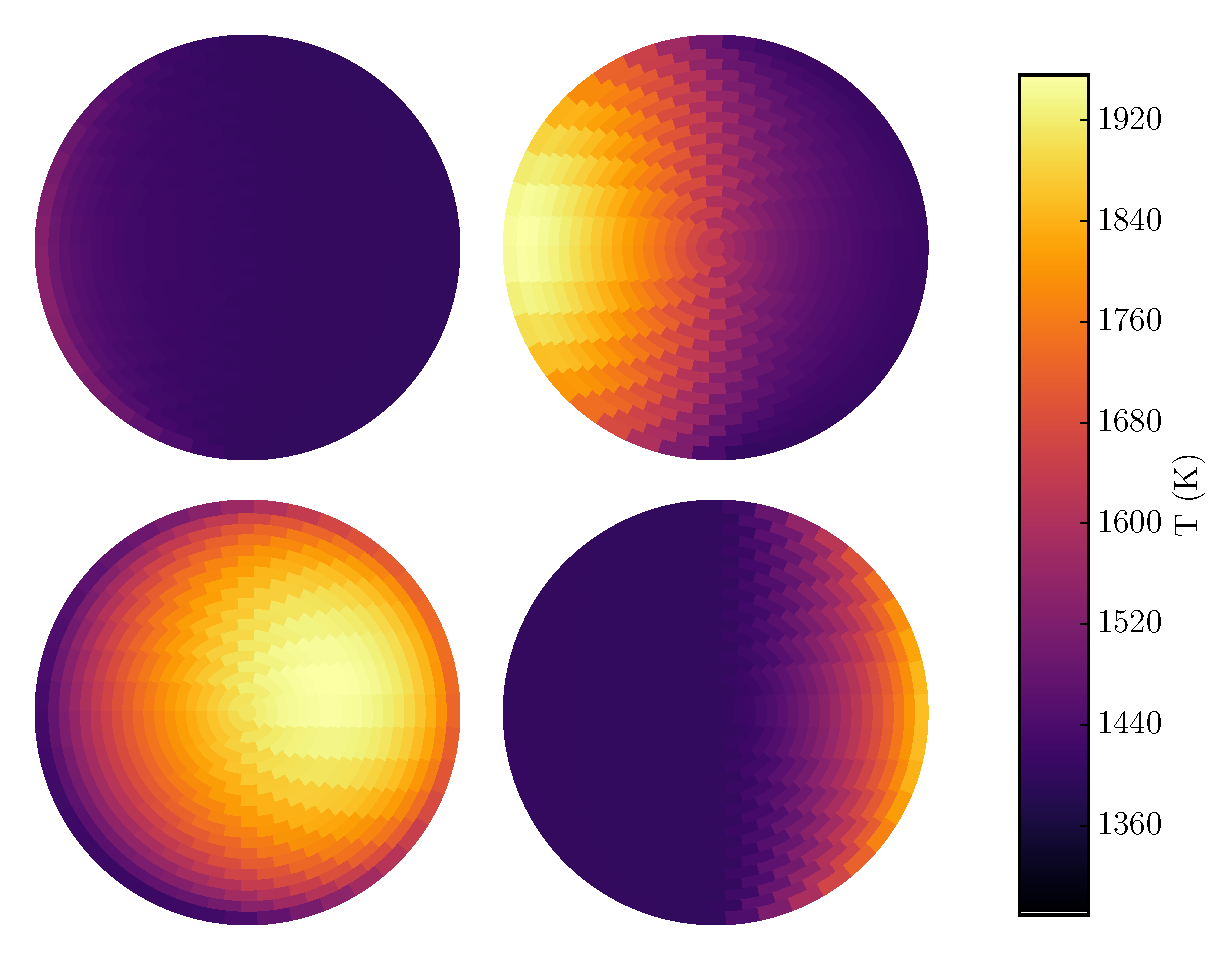
\includegraphics[width=\columnwidth]{img/free_parameterstemp_map.pdf}
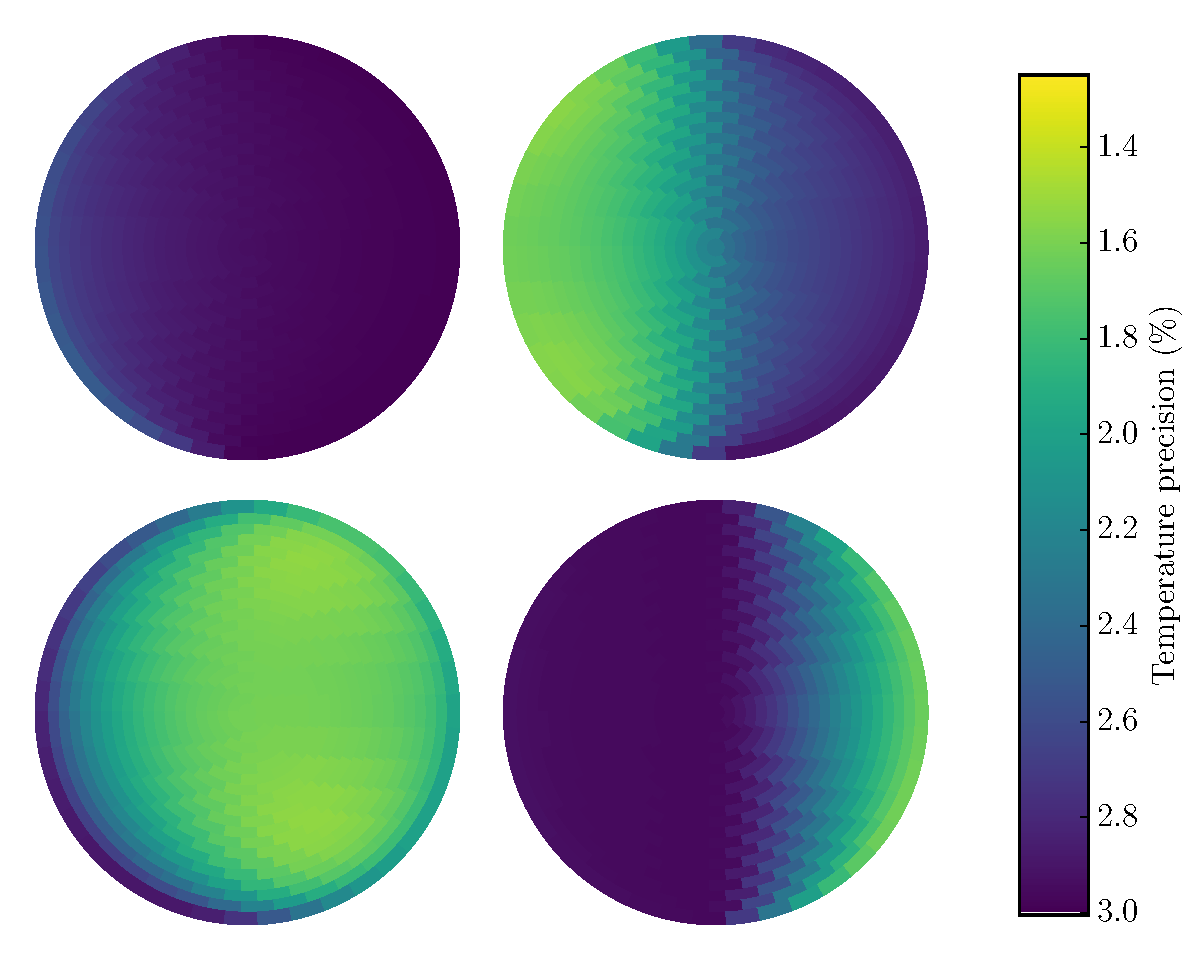
\includegraphics[width=\columnwidth]{img/free_parameterstemp_errs.pdf}
\caption{The underlying temperature distributions generated by the zhang model.}
\label{fig:extract_region}
\end{center}
\end{figure*}

\subsection{Model design}\label{sec:fitting}

The model is designed so that an arbitrary brightness distribution can be used, and that the resulting phase curve and secondary eclipse lightcurves can be calculated rapidly and accurately. 

The visible disc of the planet is divided into a series of annuli, and then these in turn are separated in theta. The number of segments in each annuli are chosen so that the area of every sector is the same. This results in 1 circular segment in the center, then 3 regions in the second annuli See the schematic in figure \ref{fig:schematic}. The planet is defined to have a radius of 1. Other grid schemes could be implemented in future versions, for example, if it is decided that the information content is higher in some parts of the planet than others then the grid could be made finer in these regions.


In practice, it is found that dividing the planet into 5 radially (25 total sectors) gives results within a few percent of higher density grids, and is significantly faster to run.

Each of the grid segments is a well defined geometric shape for which it is simple to calculate the fraction blocked by the planet passing behind the star, which in the model is represented as an occulting circle.

The area of one of these geometrical segments that has been blocked by the star can always be calculated by breaking the area into a combination of circle segments and triangles, for which the areas are known.

There are a small number of different general "cases" for the numbers of triangles and segments that must be used, that can be selected based on the number and types of "collision points" between the planet region and the stellar circle. Therefore, the first step for calculating the occulted area for each segment of the planet is to calculate these collision points. Within \textsc{spiderman} the region boandaries are stored as the radius of the inner and outer arcs, and the $\theta$ angle of the two radial lines.

Finding the collision points between an arc or a line and a circle (the star), if any exist, are trivial and fast to calculate. The code then classifies the geometric "case" of the collision based on the number of collision points on the 4 boundary sides.

For example, if there are two collision points between the outer arc and the edge of the star, then this falls into the case where the occulted area can be described by the sum of two circular segments. Other cases include larger numbers of components, but can still be described by a small number of circle segments and triangles.

The advantage of this geometric approach is that the planet can be described by a small number of regions with no loss in numerical precision, enabling eclipses and phase curves to be calculated extremely rapidly.

\begin{figure}
\begin{center}
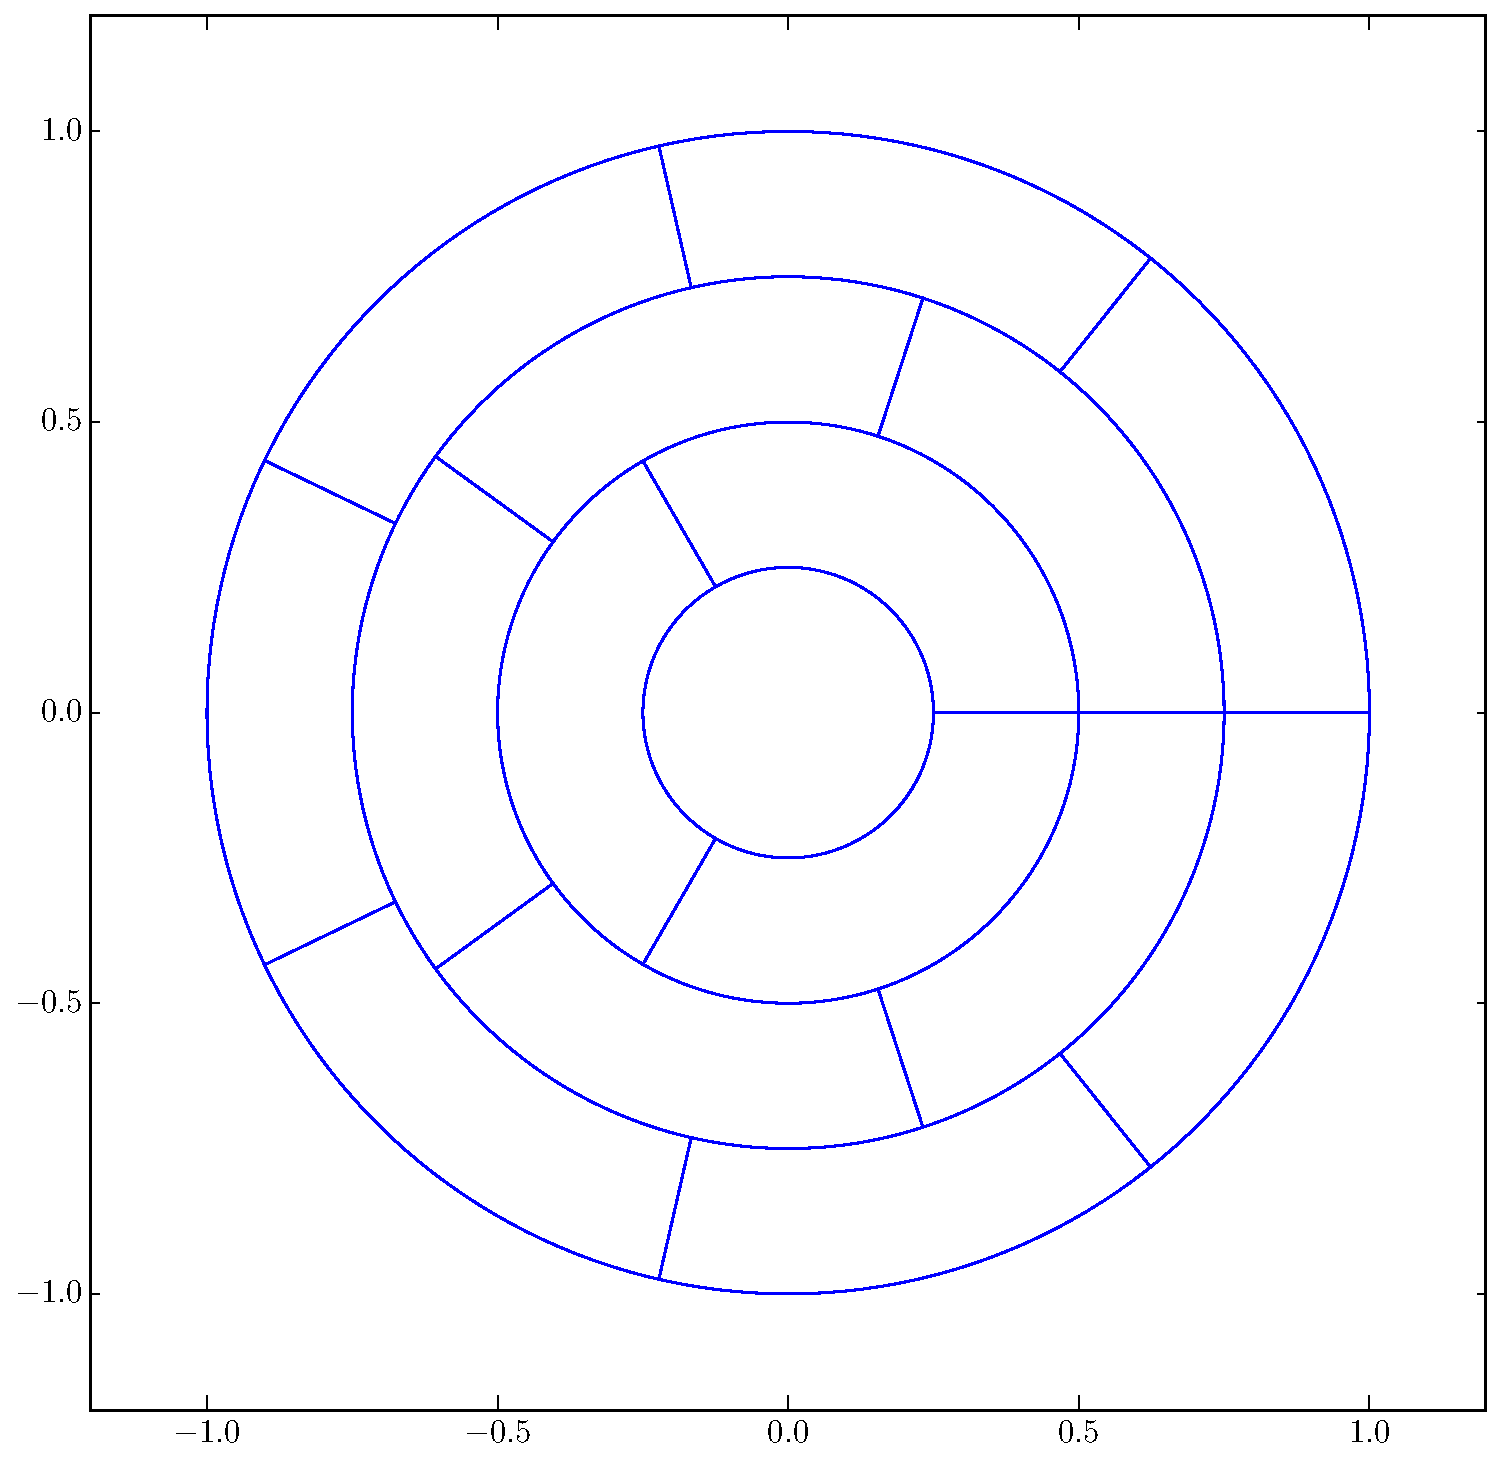
\includegraphics[width=0.8\columnwidth]{img/frame1.pdf}
\caption{Schematic representation of the planet grid. All sectors are equal area.}
\label{fig:schematic}
\end{center}
\end{figure}

\subsection{Integrator validation}\label{sec:numerical}

\begin{figure}
\begin{center}
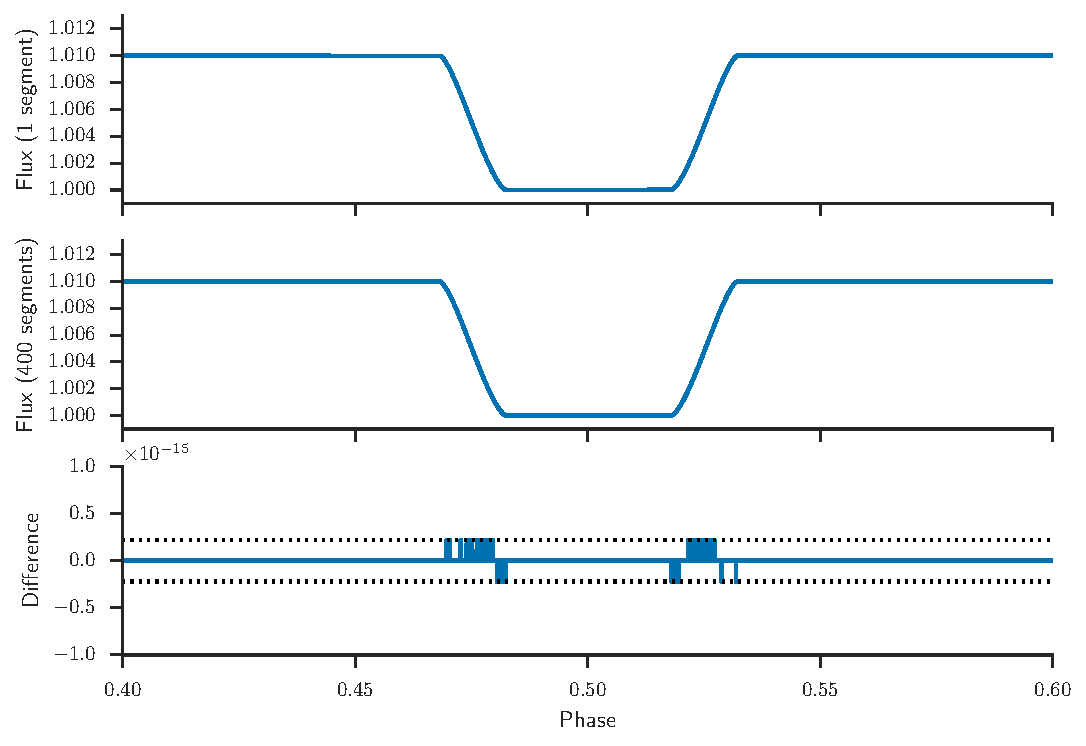
\includegraphics[width=\columnwidth]{img/precision.pdf}
\caption{This is a caption}
\label{fig:extract_region}
\end{center}
\end{figure}

\subsection{Performance}\label{sec:performance}

In typical usage, SPIDERMAN is capable of producing over 1000 models per second on a single core. This means that a 1 million MCMC sample can be generated in approximately a quarter of an hour.

The performance tests were carried out on a single core of an Intel Core I5-3470 Processor.

\begin{figure}
\begin{center}
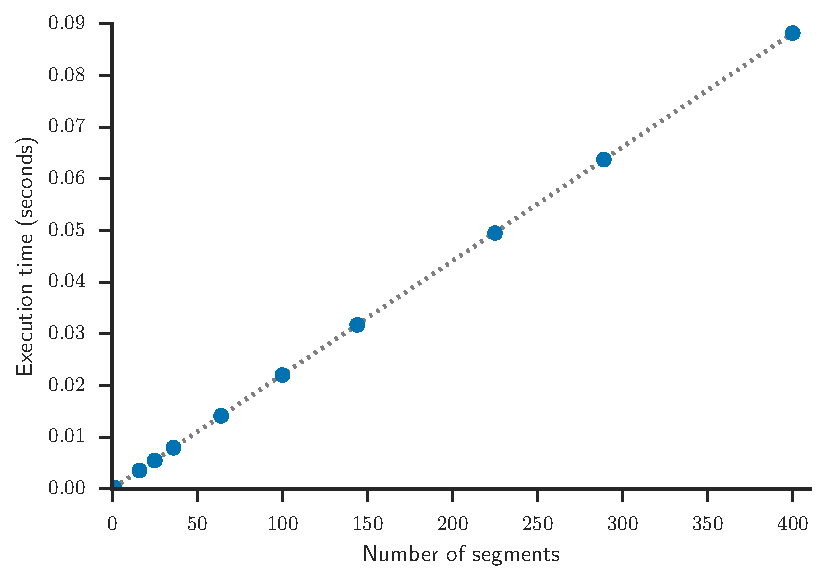
\includegraphics[width=\columnwidth]{img/exec_time.pdf}
\caption{This is a caption}
\label{fig:exec_time}
\end{center}
\end{figure}

\subsection{Available models}\label{sec:ttof}


\subsection{Temperature to fluxes}\label{sec:ttof}

Some physical models, such as the one adapted from \citep{zhang2016} are defined in terms of temperature, where of course the observable that is being fit for is the emitted flux. Therefore, it is necessary

If we make the assumption that the temperature distribution maps to the \emph{brightness temperature} distribution, then we can recover these fluxes. This will be valid for narrow

An additional factor that is not currently considered by the model but will be featured in future releases of the code is to also include the ability for the user to define instrument response functions as a function of wavelength.

\subsection{}\label{sec:ttof}

\section{The \textsc{spiderman} package}\label{sec:package}

\textsc{spiderman} is an open source project and is being actively developed on github. The code is available on PyPi, and the latest stable version can easily by installed by simply running the command 

\begin{Verbatim}[frame=single]
> pip install spiderman-package
\end{Verbatim}

Or, to access the bleeding-edge development version from github:

\begin{Verbatim}[frame=single]
> git clone https://github.com/tomlouden/SPIDERMAN
> cd SPIDERMAN
> sudo python setup.py install
\end{Verbatim}

Full installation instructions and other information are available in the documentation, at \url{http://spiderman.readthedocs.io}

\begin{figure}
\begin{center}
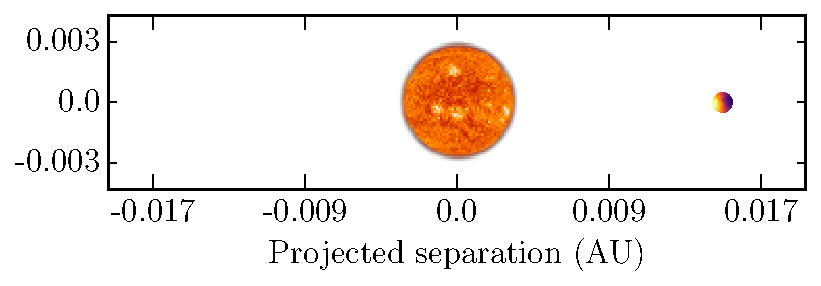
\includegraphics[width=\columnwidth]{img/system.pdf}
\caption{This is a caption}
\label{fig:extract_region}
\end{center}
\end{figure}

\section{Application to data}\label{sec:Observations}

As a test of the performance of the code the model was applied to a phase curve and secondary eclipse of WASP-43b taken with HST WFC3. These data had previously been published in \citet{Stevenson2014c}. However, in this paper the phase curve and the secondary eclipse are treated as seperate phenomena, when of course, they are both manifestations of the same underlying brightness distribution. Indeed, the bright dayside of the planet is the main driver of the phase curve, and is also the part occulted by the stellar disc. It is therefore more parsimonious, if at all possible, to use a model that accounts for both of these observations simultaneously. This also reduces the total number of paramters needed, which is satisfying from an information content angle.

One could argue that planetary limb darkening, among other effects, will act to decouple the secondary eclipse from the phase curve, and there are not good constraints on what to expect from the limb darkening as it requires a full atmosphere model treatment. \textsc{spiderman} does have the option to include planetary limb darkening, which would allow one to marginalise over the uncertainty in these parameters. 

In principle, constraints being placed on the limb darkening can constrain the vertical temperature profile of the planet, however this would require a full radiative transfer treatment of the planet.

WASP-43b appears to have a near isothermal profile \citep{Stevenson2014c}, which should correspond to a zero limb darkening. However, as I show in section X. there is a preference in the fit for a \emph{limb brightened profile} which may indicate the presence of a weak thermal inversion layer, or may simply be due to oversimplifications in the model fit.

During the MCMC fit I place the constraint that the limb darkening must be monotonic across the disc of the planet, i.e., there can be no change in the sign of the gradient. This results in profiles that are either flat, wholly limb darkened or wholly limb brightened, with no non-physically flexible profiles.

\begin{figure}
\begin{center}
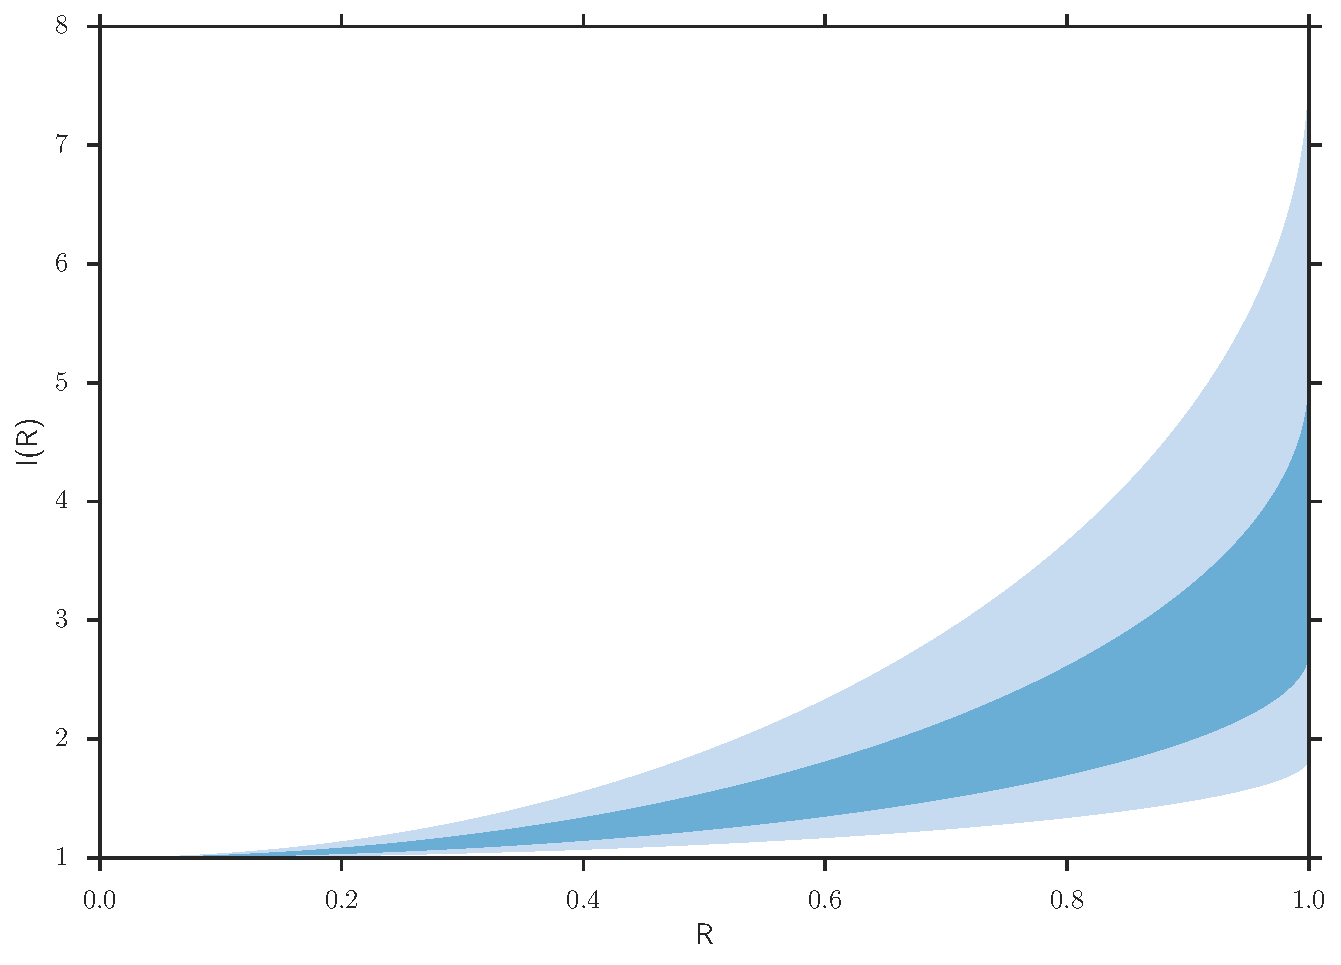
\includegraphics[width=\columnwidth]{img/ld_prof.pdf}
\caption{The 1 sigma and 3 sigma contours for the Radial intensity profile of the planet, indicating that the fit has a significant preference for limb brightened profiles }
\label{fig:limb brighten}
\end{center}
\end{figure}

\begin{figure}
\begin{center}
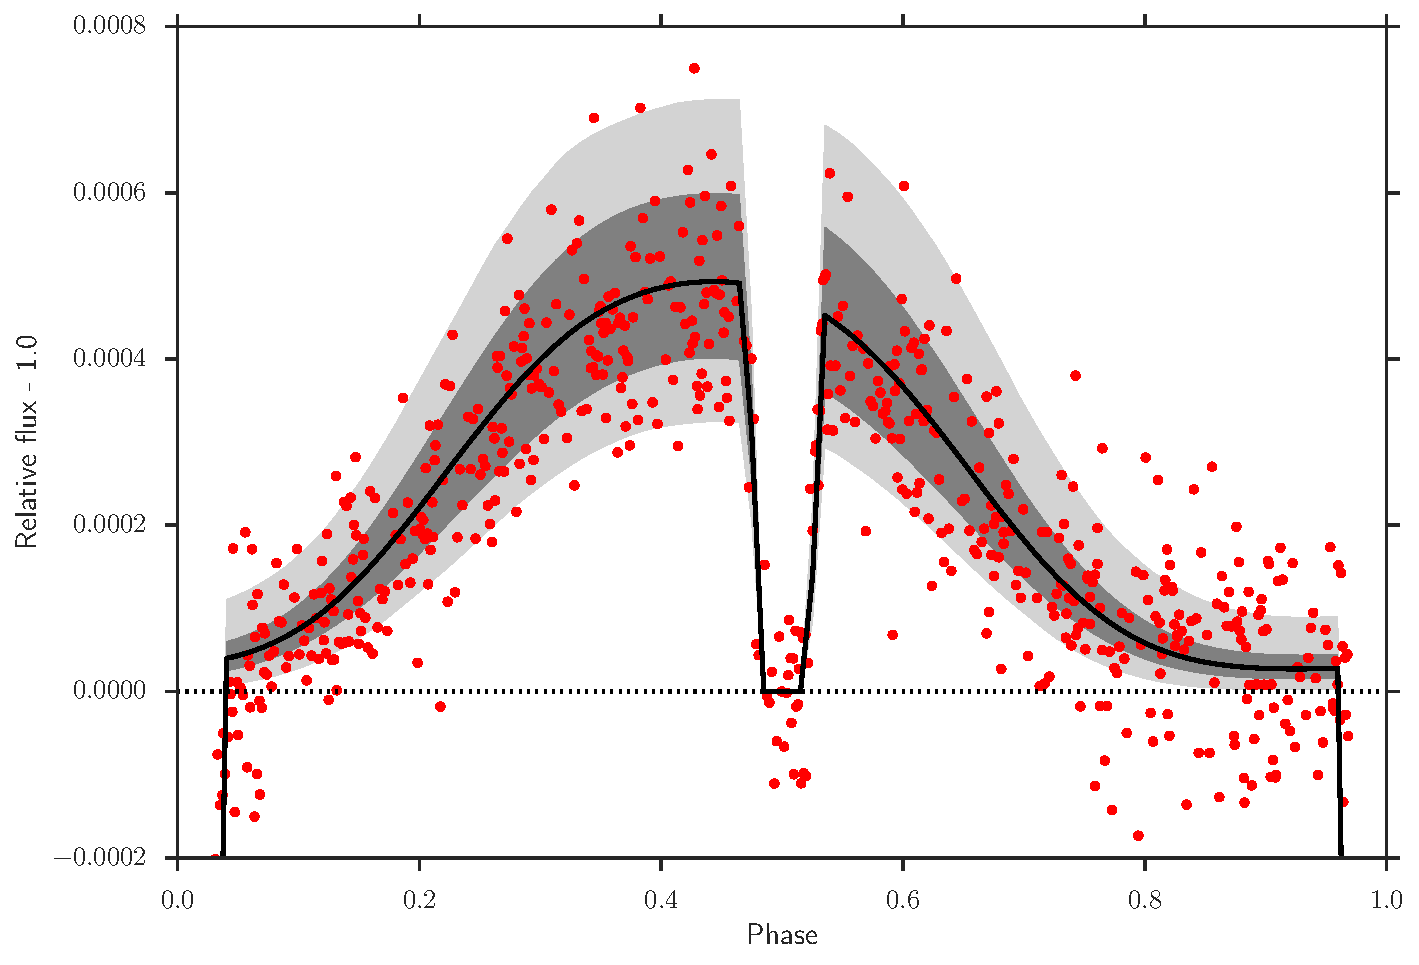
\includegraphics[width=\columnwidth]{img/model.pdf}
\caption{the uncertainty on the model from the MCMC fit. There is a greater than 3 sigma detection of night-side flux.}
\label{fig:model}
\end{center}
\end{figure}

\section{Systematics model}\label{sec:systematics}

As with most exoplanet observations with Hubble, the data are effected by the idiosyncratic systematic errors of the instrument. Fortunately, the sources of these errors are relatively well understood, and are generally quite repeatable between observations. They are therefore quite straightforward to fit for and remove. 

The systematics model is the same that was used in the previous treatment \citep{Stevenson2014c}.

In brief, there are three components to the systematics model:

1. Scan direction offset

There is an offset in the recorded flux depending on which way the the ccd was scanning during the readout, in one half of exposures the scan direction is in the same direction as the readout, and in the other half it is the offset. This leads to a very repeatable offset in the fluxes between the two scan directions, which can be captured with a single parameter "scale"

2. Orbit long "hook effect"

\begin{equation} \label{eq:hook}
F_{cor} = F*(1-exp(-r1 t_{orb}-r2-r3 \delta_{fo}))
\end{equation}

Where $F$ is the flux before correction and $F_{cor}$ is the corrected flux $t_{orb}$ is the time from the start of each \emph{obit}, $r1$, $r2$, $r3$ are the fitted coefficients. This exponential ramp has a different shape during the first orbit of a visit, so the $\delta_{fo}$ function takes a value of 1 if the orbit is the first, and 0 at all other times.

The exponential hook shape is believed to be related to charge trapping, and is a characteristic and repeatable feature across orbits, so these parameters are fit simultaneously over visits.

3. A visit long slope. 

Each visit displays a decreasing slope, which is modelled as a second order polynomial. The cause of these features is unknown, and they have not been linked to any physical parameters of the telescope \cite{Wakeford2016}. Here, they are also likely blended with the "Breathing" systematics of the instrument, which are caused by the changing thermal environment of the telescope during its orbit changing the focal length of the instrument. The shape of these visit long effects is slightly different between the three visits used here, so the three paramters of the polynomial are fit seperately for the three visits.

The feature that is the greatest cause for concern is the visit long slope in the data, as this has a comparable timescale and amplitude to the planets phase curve, so there is potential for serious degeneracies between the systematics and the physical model.

Fortunately, the phasing of the observations is such that the three visits cover very different ranges of the phase curve, which does tend to alleviate the degeneracy. As can be seen in the large corner plot in figure \ref{}, these parameters are still degenerate with the physical model parameters, in particular the $\xi$ paramter which controls the phase curve shape, but the constraints placed on these parameters are still useful, and marginalising over the systematics parameters with the MCMC should remove any doubt that the results are only an artefact.

Future analysis of this dataset could use a Gaussian process noise model instead of the parametrised one featured here, as used in (REF), this could provide further confidence in the results, as the added flexibility of the GP model and the explicit fit for the timescale of the features would allow the degeneracy to be explored with fewer explicit hyper-parameters.

\begin{figure*}
\begin{center}
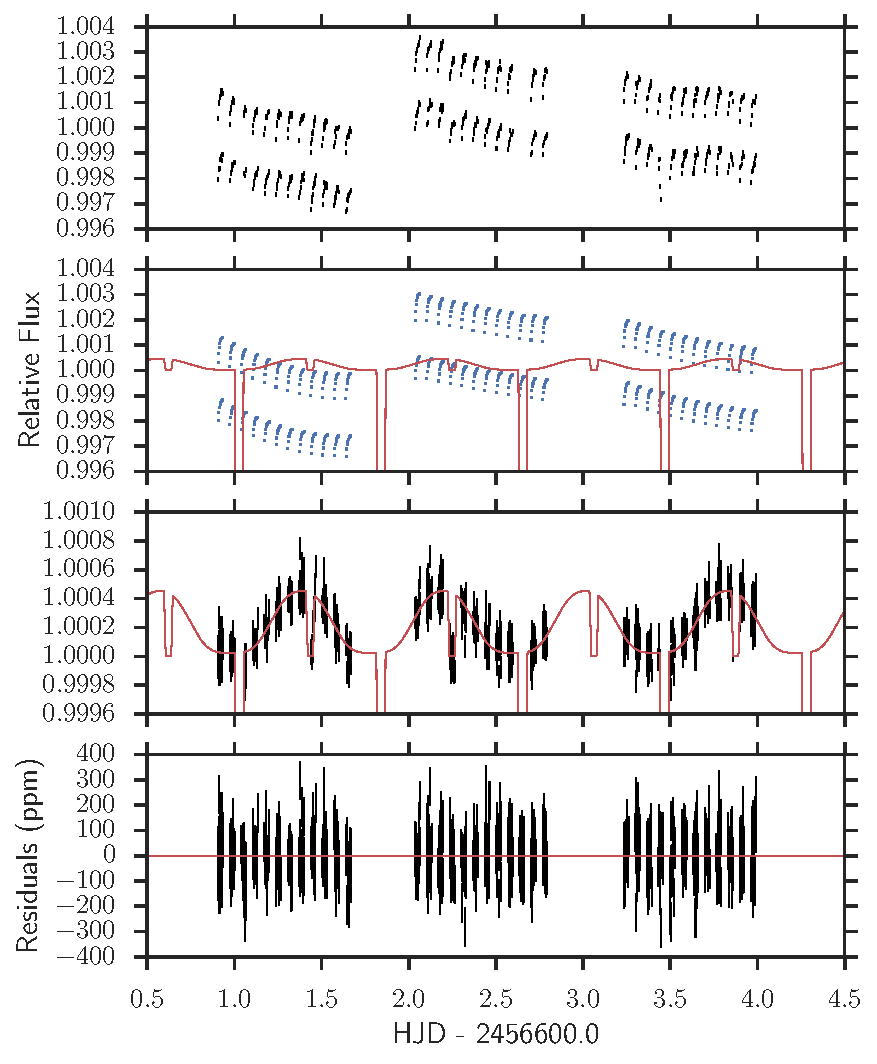
\includegraphics[width=0.8\textwidth]{img/systematics.pdf}
\caption{Top: raw data from HST, the systematic components are all visible. second panel shows the physical model fit (red) and the systematic model (blue). The third panel shows the model fit to the data with the systematic noise component removed, the fourth panel is the residuals of the fit.
}
\label{fig:systematics}
\end{center}
\end{figure*}

\section{MCMC}\label{sec:MCMC}

To investigate the correlation between the

In table \ref{tab:results}

\begin{figure*}
\begin{center}
\includegraphics[width=\textwidth]{img/huge_triangle.pdf}
\caption{stupidly big triangle plot1}
\label{fig:extract_region}
\end{center}
\end{figure*}

\begin{figure}
\begin{center}
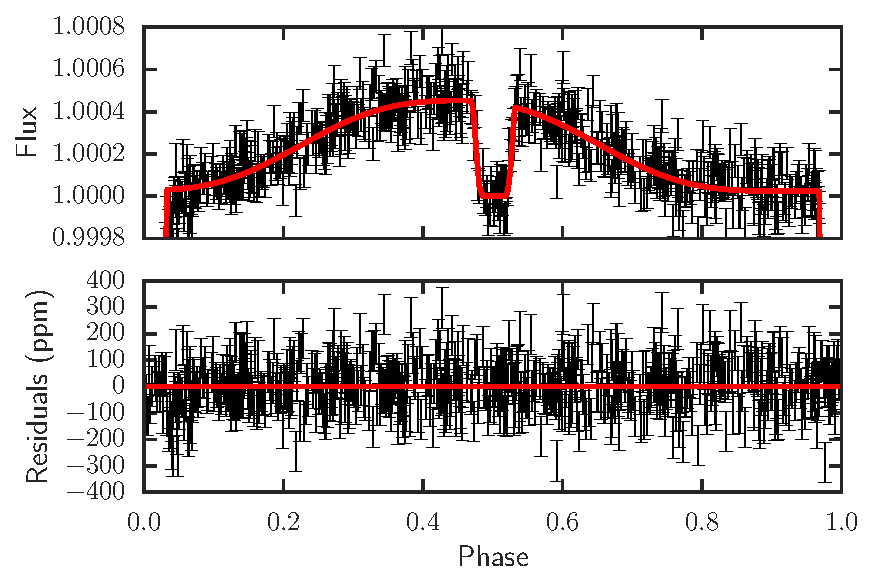
\includegraphics[width=\columnwidth]{img/new_lc.pdf}
\caption{The final fitted lightcurve. The primary transit is fit by \textsc{batman} and is off the scale of this figure.}
\label{fig:extract_region}
\end{center}
\end{figure}

\begin{center}
\begin{table*}{
\caption{This is my caption}
\begin{center}
\begin{tabular}{l c c c c c}
\hline
\hline
          &   ld fixed   &             &   ld free    &             \\
name      &   median     & error       &   median     & error        & unit        \\
\hline
Period &  0.813473977 & $\pm$ 0.000000036 &  0.813473979 & $\pm$ 0.000000034 & days\\
$t0$ & 2456601.0274024 & $\pm$   0.0000091 & 2456601.0274025 & $\pm$   0.0000091 & days\\
$a/R_*$ &       4.8762 & $\pm$      0.0089 &       4.8772 & $\pm$      0.0087 & -\\
inclination &       82.123 & $\pm$       0.038 &       82.125 & $\pm$       0.037 & degrees\\
eccentricity & 0 & - & 0 & - & -\\
$R_p/R_*$ &     0.159692 & $\pm$    0.000093 &     0.159650 & $\pm$    0.000092 & -\\
$u1$ &       0.3880 & $\pm$      0.0083 &       0.3875 & $\pm$      0.0082 & -\\
$u2$ & 0 & - & 0 & - & -\\
$c_1$ & 3.687319e+08 & $\pm$    0.000090e+08 & 3.687526e+08 & $\pm$    0.000089e+08 & -\\
$c_2$ & 3.693661e+08 & $\pm$    0.000097e+08 & 3.693654e+08 & $\pm$    0.000097e+08 & -\\
$c_3$ & 3.689717e+08 & $\pm$    0.000093e+08 &  3.68984e+08 & $\pm$     0.00010e+08 & -\\
$v1_1$ &   -1.484e+06 & $\pm$       0.045e+06 &   -1.559e+06 & $\pm$       0.049e+06 & -\\
$v1_2$ &    -6.31e+05 & $\pm$        0.50e+05 &    -6.19e+05 & $\pm$        0.55e+05 & -\\
$v1_3$ &    -8.56e+05 & $\pm$        0.49e+05 &    -8.57e+05 & $\pm$        0.54e+05 & -\\
$v2_1$ &    1.004e+06 & $\pm$       0.059e+06 &    1.076e+06 & $\pm$       0.064e+06 & -\\
$v2_2$ &     1.83e+05 & $\pm$        0.61e+05 &     1.92e+05 & $\pm$        0.67e+05 & -\\
$v2_3$ &     4.08e+05 & $\pm$        0.62e+05 &     3.77e+05 & $\pm$        0.67e+05 & -\\
$r1$ &        123.2 & $\pm$         3.5 &        122.7 & $\pm$         3.5 & -\\
$r2$ &        5.874 & $\pm$       0.011 &        5.877 & $\pm$       0.011 & -\\
$r3$ &       -0.087 & $\pm$       0.028 &       -0.113 & $\pm$       0.028 & -\\
scale &   -0.0024748 & $\pm$   0.0000061 &   -0.0024749 & $\pm$   0.0000060 & -\\
$p_{u1}$ & 0 & - &         -1.2 & $\pm$         0.9 & -\\
$p_{u2}$ & 0 & - &         -2.7 & $\pm$         1.1 & -\\
$a$ &      0.01421 & $\pm$     0.00040 &      0.01419 & $\pm$     0.00040 & AU\\
$\xi$ &        0.436 & $\pm$       0.050 &        0.417 & $\pm$       0.053 & -\\
$T_n$ &         1290 & $\pm$          39 &         1069 & $\pm$          62 & K\\
$\Delta_T$ &          699 & $\pm$          53 &          827 & $\pm$          92 & K\\
$T_s$ &         4530 & $\pm$         120 &         4530 & $\pm$         120 & K\\
\end{tabular}
\end{center}
\label{tab:results}
}
\end{table*}
\end{center}

\section{Discussion}\label{sec:Discussion}

\subsection{Future work}\label{sec:future work}

\textsc{spiderman} is still under development, and there are a number of features that are planned to be implemented:

- More thermal brightness distributions, such as orange segments and a simple parameterised hotspot (etc?)
- Implement \emph{reflected} light phase curves and secondary eclipses, through adding appropriate brightness distributions like Lambertian reflectors and patchy clouds.
- Allow calculation of multiple spectral channels simultaneously, with linked system parameters.
- Include instrument response in calculating flux ratios
- Better treatment of errors in the spectral energy distribution of the star - include errors in log-g and Metalicity

In regards to the re-analysis of WASP-43bs phase curve, future analysis will focus on

- Confirming the detected flux on the nightside is a real feature and not an artefact
- Further test for degeneracies between HST systematics and the physical model of the phase curve, in particular the combination of visit long slope and breathing modes. This could be accomplished by a Gaussian process analysis.

\section{Conclusions}

\section*{Acknowledgements}

The majority of this work was carried out at the kavli summer program in physics 2016. T.L extends his gratitude to the program organisers, in particular Jonothan Fortney and Pascale Geurard.

T.L. is supported by a STFC studentship. P.W. is supported by a STFC consolidated grant (ST/L000733/1).

%%%%%%%%%%%%%%%%%%%%%%%%%%%%%%%%%%%%%%%%%%%%%%%%%%

%%%%%%%%%%%%%%%%%%%% REFERENCES %%%%%%%%%%%%%%%%%%

% The best way to enter references is to use BibTeX:

\bibliographystyle{mnras}
%\bibliography{/home/astro/phrmat/Documents/BibTeX/Papers-LowEUV}
\bibliography{bibliography}
%\bibliography{example} % if your bibtex file is called example.bib


% Alternatively you could enter them by hand, like this:
% This method is tedious and prone to error if you have lots of references
%\begin{thebibliography}{99}
%\bibitem[\protect\citeauthoryear{Author}{2012}]{Author2012}
%Author A.~N., 2013, Journal of Improbable Astronomy, 1, 1
%\bibitem[\protect\citeauthoryear{Others}{2013}]{Others2013}
%Others S., 2012, Journal of Interesting Stuff, 17, 198
%\end{thebibliography}

%%%%%%%%%%%%%%%%%%%%%%%%%%%%%%%%%%%%%%%%%%%%%%%%%%

%%%%%%%%%%%%%%%%% APPENDICES %%%%%%%%%%%%%%%%%%%%%

%\appendix

%\section{Some extra material}

%If you want to present additional material which would interrupt the flow of %the main paper,
%it can be placed in an Appendix which appears after the list of references.

%%%%%%%%%%%%%%%%%%%%%%%%%%%%%%%%%%%%%%%%%%%%%%%%%%


% Don't change these lines
\bsp	% typesetting comment
\label{lastpage}
\end{document}

% End of mnras_template.tex